\documentclass[t,12pt]{beamer}

\usepackage[T1]{fontenc} 
\usepackage[frenchb]{babel}
\usepackage[utf8]{inputenc}

\usetheme{JuanLesPins}
\usecolortheme{beaver}

\title{Exportation de notes prises sur un Sony PRS-T1}
\author{Grégory Putz, Ahma Bekele, Mathieu Bivert}
\date{\oldstylenums{Juin 2012}}
\begin{document}
\frame{\titlepage}

\begin{frame}
$\vcenter{
\begin{figure}[!ht]
  \vfill
  \centering
  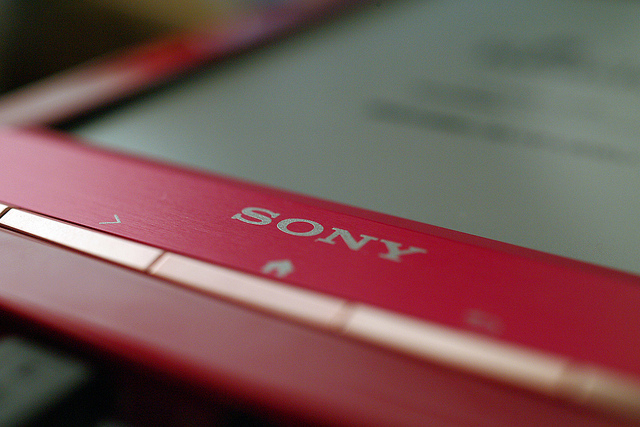
\includegraphics[scale=1]{prs-t1.png}
\end{figure}}$
  \tableofcontents
\end{frame}

\begin{frame}
  \frametitle{An Ebook-reader}
  Advantages of a reader over a bookcase:
  \begin{itemize}
    \pause \item portable, light;
    \pause \item economical/ecological (nowadays, paper is mainly manufactured from trees…);
    \pause \item non-destructive note taking;
    \pause \item files and notes sharing;
    \item etc.
  \end{itemize}
  \pause Notably usefull for researchers, avid readers, etc.
\end{frame}

\begin{frame}
  \frametitle{Problematic}
  \begin{itemize}
  \pause \item Sharing notes;
  \pause \item No standardized note taking format.
  \pause \item Notes stored  on the ebook:
    \begin{itemize}
      \item half in SQLite;
      \item half in XML (SVG).
    \end{itemize}
  \pause In a nearly wholly comprehensible format.
  \pause \item client requests program to run GNU/Linux,
  \pause Sony software is closed source, windows only (although
  it may run on wine, XXX check §).
  \end{itemize}
\end{frame}

\begin{frame}
  \frametitle{Notes format}
  \begin{itemize}
    \item PDF standard defines Annotations (§ 8.4);
    \pause \item Java classes to manipulate PDF (eg. Qoppa (commercial),
      iText (open source, free and commercial)), including annotations;
    \pause \item different formats to annotate document (PDF, Epub, etc.)
      depending on the software (Okular, Xournal, etc.), with a possibility to
      export in PDF.
  \end{itemize}
\end{frame}

\begin{frame}
  \frametitle{A solution}
  \begin{itemize}
    \item in Java (portability) and ease of developpment (pre-existing
      librairies, etc.);
    \pause \item with iText for PDF manipulation (free, open);
    \pause \item console and graphical (SWT, portability) interfaces;
  \end{itemize}
\end{frame}

\begin{frame}
  \frametitle{Diagram}
  \begin{figure}[!ht]
    \vfill
    \centering
    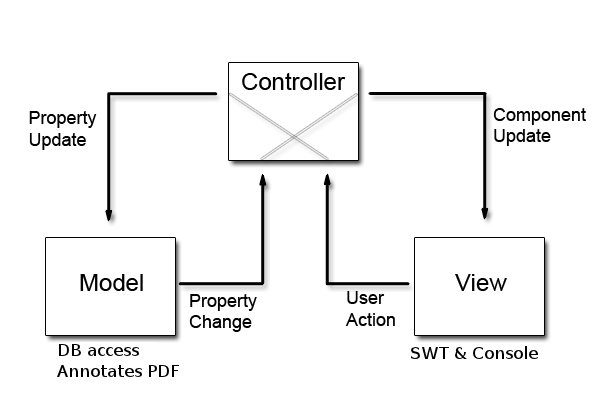
\includegraphics[scale=.5]{diagram.png}
  \end{figure}
\end{frame}

\begin{frame}
  \frametitle{Demonstration!}
\end{frame}

\end{document}
